\chapter{Discussion}


\section{Oscillations (Working Title)}

The results in section \ref{sec:reducing_stepsize} show that when the stepsize is reduced, the oscillations in the states increase. This phenomenon is also present when using a stepsize of $0.2$s, but because of the longer time between every re-initiation the effect is not as visible as for $0.1$s.

A major contributor to generating these oscillations is the trajectory generator described in section \ref{subseq:generating_trajectory}, that assumes the UAV will maintain a fixed speed in order to calculate the distance the UAV will travel during one timestep. This assumption will introduce some inaccuracies, but the results show that during the optimization the speed did not vary much. However, this method of generating the trajectory introduces another inaccuracy, in that the path given as an input is discretized.

Since the reference path is discretized, it is not possible to always find a point up ahead that is excactly the distance the UAV will travel during one timestep away. For this reason, points with a distance away that is within a given range is accepted as the next waypoint. If this range is too big the inaccuracy will be too big, which will cause a spike in the reference model in the cost function. Because of this spike in reference the optimization algorithm will seek to follow the spike, which causes the oscillations in the states.

\begin{figure}[]
	\centering
    \makebox[\textwidth][c]{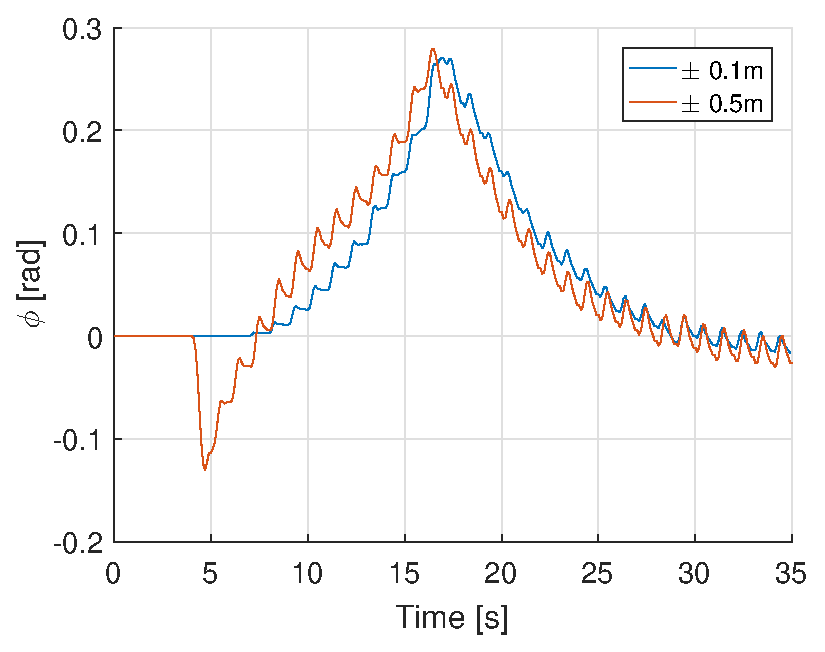
\includegraphics[width=0.8\textwidth, keepaspectratio=true]{../../results/opt/error/fig/attitude.eps}}
	\caption{The roll angle of the aircraft during a linear $45\degree$ turn with different acceptance rates for waypoints.}
	\label{fig:oscillating_attitude}
\end{figure}

In Figure \ref{fig:oscillating_attitude} the effect the acceptance range of waypoints has on the roll through a $45\degree$ linear turn is shown. When the acceptance range is $\pm 0.5$m, the magnitude of the oscillations is bigger than for an acceptance range of $\pm 0.1$m. A part from a spike in the wrong direction for the $\pm 0.5$m signal, the two roll angles follow approximately the same trajectory.


\section{Comment on Control Signals}


\section{Cost Function}